\section{Combative Strategies}
\label{overview}

Cloud services introduce new security threats into the world of computing, ones that render classical computing security measures partially, and in some cases entirely, ineffective. The three mediums which cloud technologies are accessible through SaaS, PaaS, and IaaS each lend themselves to differing levels of vulnerability.\cite{theoharidou}\cite{subashini} When combating any threat, whether it be a classical computing threat or a threat unique to cloud systems, there is two types of strategies which are employed.

Detection strategies are the last line of defense against any attack on a computer system. The ability to detect a compromised segment of the system is crucial if one is to combat and terminate the threat. The administrator threat is one which is particularly difficult to detect, as the perpetrator of such an attack has the access level of a system administrator giving the attacker the ability to traverse the systems undetected. The methods employed to detect an administrator attack have to be implemented across the all infrastructure of the cloud system.\cite{dawoud}

Prevention strategies are ones which are common to both classical and cloud computing such as cloning, encryption, migration, deletion. Although the strategies may differ slightly in their application depending on the domain, the general idea behind them is the same (see figure \ref{prevention_detection_image}).
This section will explore the medium which is most vulnerable to the administrator threat, and the techniques that can be used to prevent against and detect the threat.

\begin{figure}
  \centering
    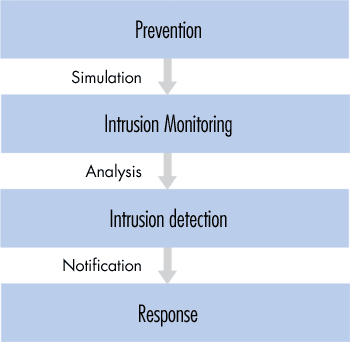
\includegraphics[height=3.5cm, width=4cm]{logging}
  \caption{Progression of a prevention and detection strategy to protect against administrator threats}
  \label{prevention_detection_image}
\end{figure}

\subsection{Higher Level Infrastrcutre}
\label{hlInfrastructure}

The infrastructure of any computer system is the base on which its entire set of applications must rely. If the infrastructure would be compromised the integrity of every application would be lost. \cite{dawoud} It is then clear that having a solid infrastructure is integral to the security of the software system as a whole. The research community has realized this and thus the majority of research has been on supplying techniques that secure on commodity hardware infrastructure. The next sections will discuss the three main techniques used to protect the integrity of the infrastructure as a whole.

\label{hlLogging}

\textbf{Logging} has been used by computer programmers as the looking glass into the brain of a computer. It allows a programmer to see the execution of their program which gives them insight on how the software is working and what functions are being performed. This is the same idea behind detecting an administrator attack. Logging can be seen as a preventative measure against insider attacks as it provides a deterrent to those thinking of steal customer information although it is employed as more of a detective feature of software systems.\cite{sirer} Just as a computer programmer wants to follow the execution of a program, logging of system access creates a path that can be followed to detect misuse of power through the system.

Logging on its own is not much help unless there is something to realize when a misuse of power has occured.\cite{althebyan} There have been may systems developed to take advantage of the bread crumbs left behind in the form of log files. In general these systems build a knowledge over time of user patterns, then if one of these patterns ever deviates there is a chance of a leak, MIDAS is one of these systems. MIDAS or Monitoring Intrusion Detection Administrator System, is a type of Big Brother system which has a global overview of all actions which occur on the system.\cite{nguyen} Some other systems which employ the same relative strategy as MIDAS are NSM, DPEM, the latter mentioned systems are more directed at network security and unix process security respectfully. Many of the systems mentioned above are currently being used and some are offered as open source works, but there is no research available into the effectiveness of these systems. The idea of tracing the paths which programs, users, and network packets take is not a new idea, but it has been repurposed to monitor and maintain a secure infrastructure in cloud software systems.\cite{nguyen}\cite{mukherjee}


\label{hlSecureHW}

\textbf{Secure Hardware :} Digging a little deeper into system infrastructure, the lowest level of defense against administrator attacks is directly built into the hardware. Secure hardware is an area of research which is gaining steam in the hardware, especially the processor, manufacturing field. In particular there are two hardware components that are targets of data theft and hacking, that is RAM and the CPU. The nature of these components as memory storage and computational units make them good targets for insiders to execute unsafe code, or modify the memory or execution of a running process. Intel has combated this in part by developed a technology which they have termed Intel SGX.\cite{baumann} SGX allows for isolated execution by providing a cache, called the Enclave, which is locked during execution from all other resources. This allows for a process to run without interruption from other unsafe or unauthorized process. This type of technology would allow for specified processes to be safely hidden from even the most privileged users subsequently eliminating the chances for an insider to attack. Microsoft has picked up on this new technology and plans to implement it along with some other forms of cloud data security in their cloud protection system termed Haven. Havens' main security will be the isolated execution property of Intel SGX enabled chips.\cite{baumann}

One of the novel ideas which drives the secure hardware implementations is that of untrusted hardware components, and possibly untrusted operating systems.\cite{suh} There have been many successful distributed storage systems built on the premise that all contributing machines are untrustworthy, namely Google's distributed file system GFS, but this idea has not yet been applied at the lower levels of computer systems, until now. Although these systems are only in the design phases their ideas of limiting system knowledge to contributing parties may lead to less vulnerable systems. AEGIS is a system which proposes these ideas of untrusted hardware, by designating parts of the operating system as secure. This idea which they call the SKernel, or secure kernel, limits the amount of system knowledge that is shared between computer components.\cite{suh} AEGIS also provides what they call Tamper Evident computing capabilities, which will inform the user of any malicious activity.

The importance of a solid infrastructure is becoming clearer, and it can be seen that using the latter technologies mixed with logging a robust, secure remote computing platform is attainable.

\label{hlHoneyPots}

\begin{figure}
  \centering
    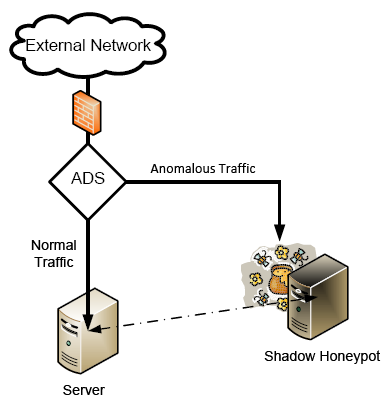
\includegraphics[width=\linewidth]{honeypots}
  \caption{An simple example of a networking with a HoneyPot sever.}
  \label{honeypot_image}
\end{figure}

\textbf{HoneyPots} are an important technology when it comes to detecting administrator or insider threats. They give the ability for data to be gathered on the attacker as the attack is being performed. This is the key to the HoneyPots technology, they act as counterfeit files, computers, networks, etc. and in order for them to be efficient there must be an attack on any of these imitations ( see figure \ref{honeypot_image} for an example HoneyPot setup ). \cite{spitzner} Than one risk when using HoneyPot systems is the other instances of HoneyPot systems are linked together, and the attack may be able to feed it false information. This system focuses on protecting the infrastructure of a system, and is a valuable tool as long as the insiders continue to use the HoneyPot instances. \cite{spitzner}

\subsection{Lower Level Infrastructure}
\label{llInfrastructure}

When an insider is attacking a system they are looking to gather information on the client or the clients machine, or deny availability to the clients resources. \cite{kandias} This then gives specific components of a machine that will be likely targets of insider attacks. This next section will delve into the classical computing methods and how they can be used to prevent successful insider attacks. Each section will look at preventing attacks directly to a machines RAM, persistent memory, and other virtual machines. The techniques are simple methods developed for classical computing and are being modified to fit the needs of cloud software systems. Each section below assumes that there is always come threat to the data which make these techniques worth implementing. It must also be noted that since these techniques have been borrowed from classical computing and are logical steps in preventing attacks on user data, no system specifically mentions use of them. \cite{szefer}

\label{llEncryption}

\textbf{Encryption} has been a known technique for protecting data, and the use of this dates back to before World War II and the use of the enigma machine. This technique is still a good preventative measure to protect against data theft. To make the most out of encryption both the cloud service provider and service user must encrypt parts of their respective systems. \cite{kandias} Encryption done by the service provider only is not enough protection from the dishonest administrator, since the encryption keys and process are available knowledge to the insider. The real benefit of encryption results when the user encrypts all her data that is on the cloud hosted services. \cite{kandias} As long as the encryption key is stored only on a non-cloud user machine the encryption will be just as safe as on a classical computing device. The downside to work with encrypting data is that it is computationally exhaustive, especially when working with the encryption of RAM. \cite{szefer}

\label{llCloning}

\textbf{Cloning} is another useful technique taken from classical computing security models. It is less usefule on classical machines other the for the use of restoring a machines state, and it can be quite physically exaustive without the use of cloud technologies to copy all the entire system over to a seperate storage device. From the point of view of the user cloning seems tedious and just as useful as on a classical machine. The benifit comes when implemented by the cloud service provider. \cite{kandias} The general idea is the more data that is cloned and relocated, the less likely and employee or attacker will know of the specific location of the data which they seek. Not to say the threat is entierly eliminated but with frequent use of the cloning technique and relocation of data it becomes harder for the insider to locate the target data. \cite{szefer} This type of technique is not very useful when dealing with RAM, and very helpful when dealing with entire virtual machines and persistent memory.

\label{llMigration}

\textbf{Migration} is a technique which relocates memory to different locations, be it different geological locations or virtual memory locations. This type of relocation technique can be applied to persistent memory and clones of virtual machines. It is most useful when it is applied by the cloud service provider. \cite{kandias} Migration can be seen as a security measure that is implemented alongside cloning, this pair of security mechanisms create a dynamic state of storage for virtual machines or persistent memory. This then limits the availability of data for malicious insiders to get a hold of. These type of techniques are especially attractive to cloud users as they can be abstracted away from the user. \cite{szefer} As mentioned above migrations effectiveness against insider attacks is the same as that of the cloning technique, and in fact migration becomes most effective when paired with multiple security techniques.

\label{llDeletion}

\textbf{Deletion} is a pretty self explanatory prevention method when it comes to any threat in classical or cloud computing. Simply put if the data is not present there is nothing to be stolen. \cite{kandias}\cite{subashini} The most useful way to implement deletion would be in conjunction with security measures such as cloning and migration. \cite{szefer} It can also be used on its own to flush and data in RAM which administrators may have access too. This technique, although its possible to implement in classical computing, really is only useful in the context of multi-user cloud computing systems. This technique can be implemented by either the service provider or the user of the cloud services. The only danger when having a sole implementation by the service provider is that the deletion schedule may be altered by the malicious administrator. \cite{sabahi}
